\section{HellfireOS}
\label{sec:HellfireOS}
O HellfireOS é um sistema operacional de tempo real preemptivo que é parte constituinte
do Hellfire System (HFS). Projetado para sistemas MPSoC, possui gerenciamento
dinâmico de tarefas que conta com a proteção contra inversão de prioridades. Seu escalonador
possui as seguintes políticas de escalonamento: Rate Monotonic, Round Robin, Earliest Deadline First e Deadline Monotonic.

Dentre as bibliotecas mais relevantes ao desenvolvimento da integração abordada na seção~\ref{sec:HAC},
consta uma LibC customizada e a biblioteca matemática (math.h) com emulação de número de ponto
flutuante. Outro ponto de interesse, nesse caso para a prova de conceito, é observarmos
que o HellfireOS não possui todas as camadas de rede implementadas, forçando a criação
ou das camadas faltantes, ou de outra solução, para possibilitar a integração.

A API do hellfire é dividida em 5 (cinco) grupos: Manipulação de Tarefas, Exclusão Mútua,
Manipulação de Memória, Comunicação entre Processos e LibC.

\begin{figure}[H]
	\centering
		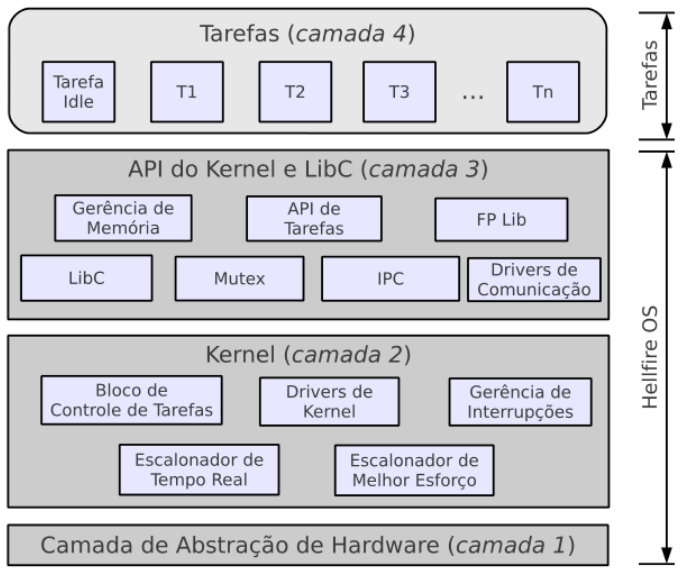
\includegraphics[width=0.5\textwidth]{fig/HellfireArch.png}
	\caption{Arquitetura em alto nível do HellfireOS.}
\end{figure}

O Hellfire System conta também com uma plataforma para design que compreende diferentes
níveis de abstração, partindo de aplicações escritas em C, até a prototipação em FPGAs.
Isto é possível graças as ferramentas e módulos que fazem parte do Hellfire Framework (HellfireFW).

O Hellfire Framwork apresenta um fluxo para o design de MPSoC baseado em sistemas embarcados do tipo crítico
como equipamentos uso médicos, dispositivos de segurança e sistemas de aeronaves. Este tipo de sistemas
apresenta uma necessidade específica de design, englobando preocupações especiais em relação à consumo de
energia e alta performance mantendo o processamento de tempo real~\cite{5450495}.
